Le \textbf{bruit de Perlin} est très utilisé dans la génération d'image. Développé par Ken Perlin en 1985, il a depuis largement été repris par toutes sortes d'industries afin de générer, entre autres, des rendus topographiques.	Il permet en effet de remplir une matrice de N dimensions (dans notre cas 3), ce qui se traduit par une élévation de sommets et un rendu graphique cohérent. Nous avons donc implémenté un algorithme de afin de générer ce bruit de Perlin. 

L'algorithme se divise en deux temps :

\begin{enumerate}
	\item Initialisation
	\item Calcul
\end{enumerate}

La phase d'initialisation consite à avoir un tableau de 512 éléments bien mélangés compris entre 0 et 255. Ensuite, le tableau se répète à partir de la valeur 256 (tab[0] = tab[256], et ainsi de suite). 

La phase de calcul est plus compliquée, car elle se découpe en plusieurs étapes. Le principe de l'algorithme est de retourner une même valeur en fonction d'un x, d'un y, et d'un z donné. On place x, y , z dans l'intervalle [0;255] avec un "et" logique. Ensuite on calcule les coordonnées en gradient du cube dans l'espace. Enfin, on calcule la valeur de retour. 

Afin de générer aléatoirement un monde virtuel, il est necessaire de remplir le tableau aléatoirement à chaque démarrage du projet. Sinon on obtiendra toujours la même monde carte, car le tableau de permutation reste toujours le même entre deux chargements.

<<<<<<< HEAD
A noter que Ken Perlin a ensuite amélioré cet algorithme, afin qu'il soit plus performant en terme de calcul et de résultat. Publiée en 2001, cette version s'appelle le bruit de Simplex.
=======
Voici le monde que l'on a reussi à généré :

\begin{center}
	\null\vspace{0.25cm}
	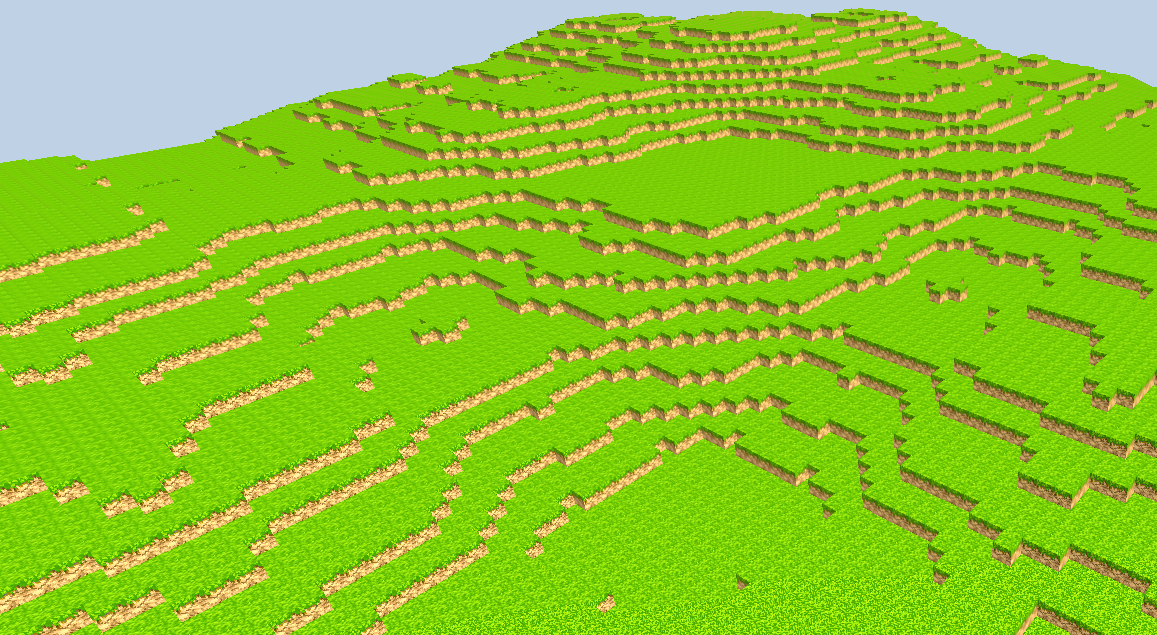
\includegraphics[height=3cm]{images/OurMinecraftWorld.png}\\
	\textit{Monde que l'on a généré à partir de l'exemple de l'API three.JS}\\
\end{center}
>>>>>>> 422a6537355f0e9f0f60acedf875af3f643e6be3
